
\section{Backbone fitting}

Evaluering af metoden med kørsel på diverse kendte proteiner og
proteiner fra Rasmus

In our experience, a good value of $w$ is around 10 since a lookahead of 10 amino acids is sufficient to avoid good local conformation that lead to an unfavorable global conformation.
\begin{figure}
	\centering
	\hspace*{-3.5mm}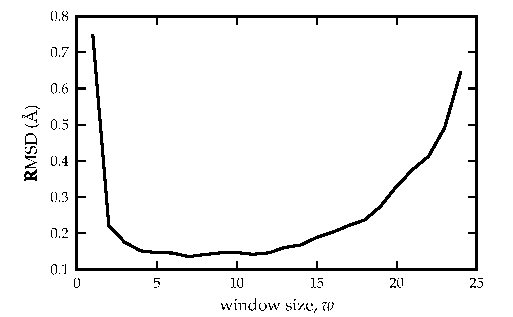
\includegraphics[width=1.1\columnwidth]{figures/plot_rmsd}
	\caption{woop}
\end{figure}

\begin{figure}
	\centering
	\hspace*{-3.5mm}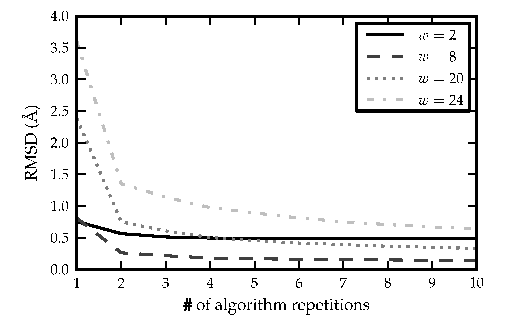
\includegraphics[width=1.1\columnwidth]{figures/plot_rmsd_convergence}
	\caption{woop}
\end{figure}

\begin{figure}
	\centering
	
\includegraphics[width=0.9\columnwidth]{figures/plot_ramachandran}
	\caption{woop}
\end{figure}


\section{Side-chain handling}
\begin{figure}
	\centering
	\hspace*{-3.5mm}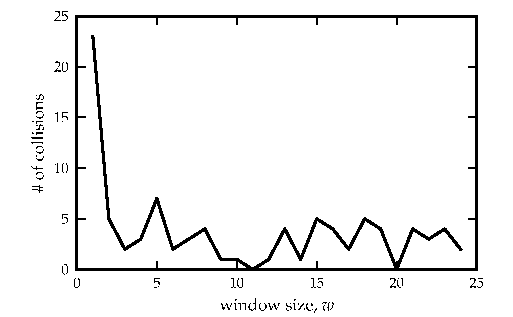
\includegraphics[width=1.1\columnwidth]{figures/plot_collisions}
	\caption{woop}
\end{figure}


%TODO billede af foldet backbone med \Ca trace
%TODO ramachandran-plot


